%%%%%%%%%%%%%%%%%%%%%%%%%%%%%%%%%%%%%%%%%
% Beamer Presentation
% LaTeX Template
% Version 1.0 (10/11/12)
%
% This template has been downloaded from:
% http://www.LaTeXTemplates.com
%
% License:
% CC BY-NC-SA 3.0 (http://creativecommons.org/licenses/by-nc-sa/3.0/)
%
% Adapted by: Romenig da Silva Ribeiro, 2014. 
% Laboratory of Informatics in Education (LInE)
% University of S�o Paulo - Instituto de Matem�tica e Estat�stica
% (romenig@gmail.com)
% 
%%%%%%%%%%%%%%%%%%%%%%%%%%%%%%%%%%%%%%%%%

%----------------------------------------------------------------------------------------
%	PACKAGES AND THEMES
%----------------------------------------------------------------------------------------

\documentclass{beamer}
\mode<presentation> {
	\usetheme{Madrid}
}
\usepackage{graphicx} 
\usepackage{booktabs}
\usepackage[brazil]{babel}
\usepackage[latin1]{inputenc}

%----------------------------------------------------------------------------------------
%	TITLE PAGE
%----------------------------------------------------------------------------------------
\title[www.usp.br/line]{Programming web-course analysis: how to introduce computer programming?}
\author[Romenig, Tulio, Le�nidas and Anarosa]{Romenig Ribeiro\inst{1},  Tulio Faria\inst{2}, Le�nidas Brand�o\inst{1} and Anarosa~Brand�o\inst{3}} 
\institute[] 
{
\inst{1}{Institute of Mathematics and Statistics - IME - USP}\and
\inst{2}{School of Arts, Sciences and Humanities - EACH - USP}\and
\inst{3}{Polytechnic School - USP}
 \\ % Your institution for the title page
\medskip
\textit{\{romenig, leo\}@ime.usp.br, tuliofaria@usp.br, anarosa.brandao@poli.usp.br} % Your email address
}
\date[FIE 2014] % (optional)
{Frontiers in Education, October 2014}
\titlegraphic{
\includegraphics[width=1.6cm]{usp.png}\hspace*{4.00cm}~%
   
\includegraphics[width=2cm]{line.png}
}
\begin{document}
%------------------------------------------------
\begin{frame}
\titlepage % Print the title page as the first slide
\end{frame}
%------------------------------------------------

\begin{frame}
\frametitle{University of S�o Paulo}
\begin{figure} %IME%
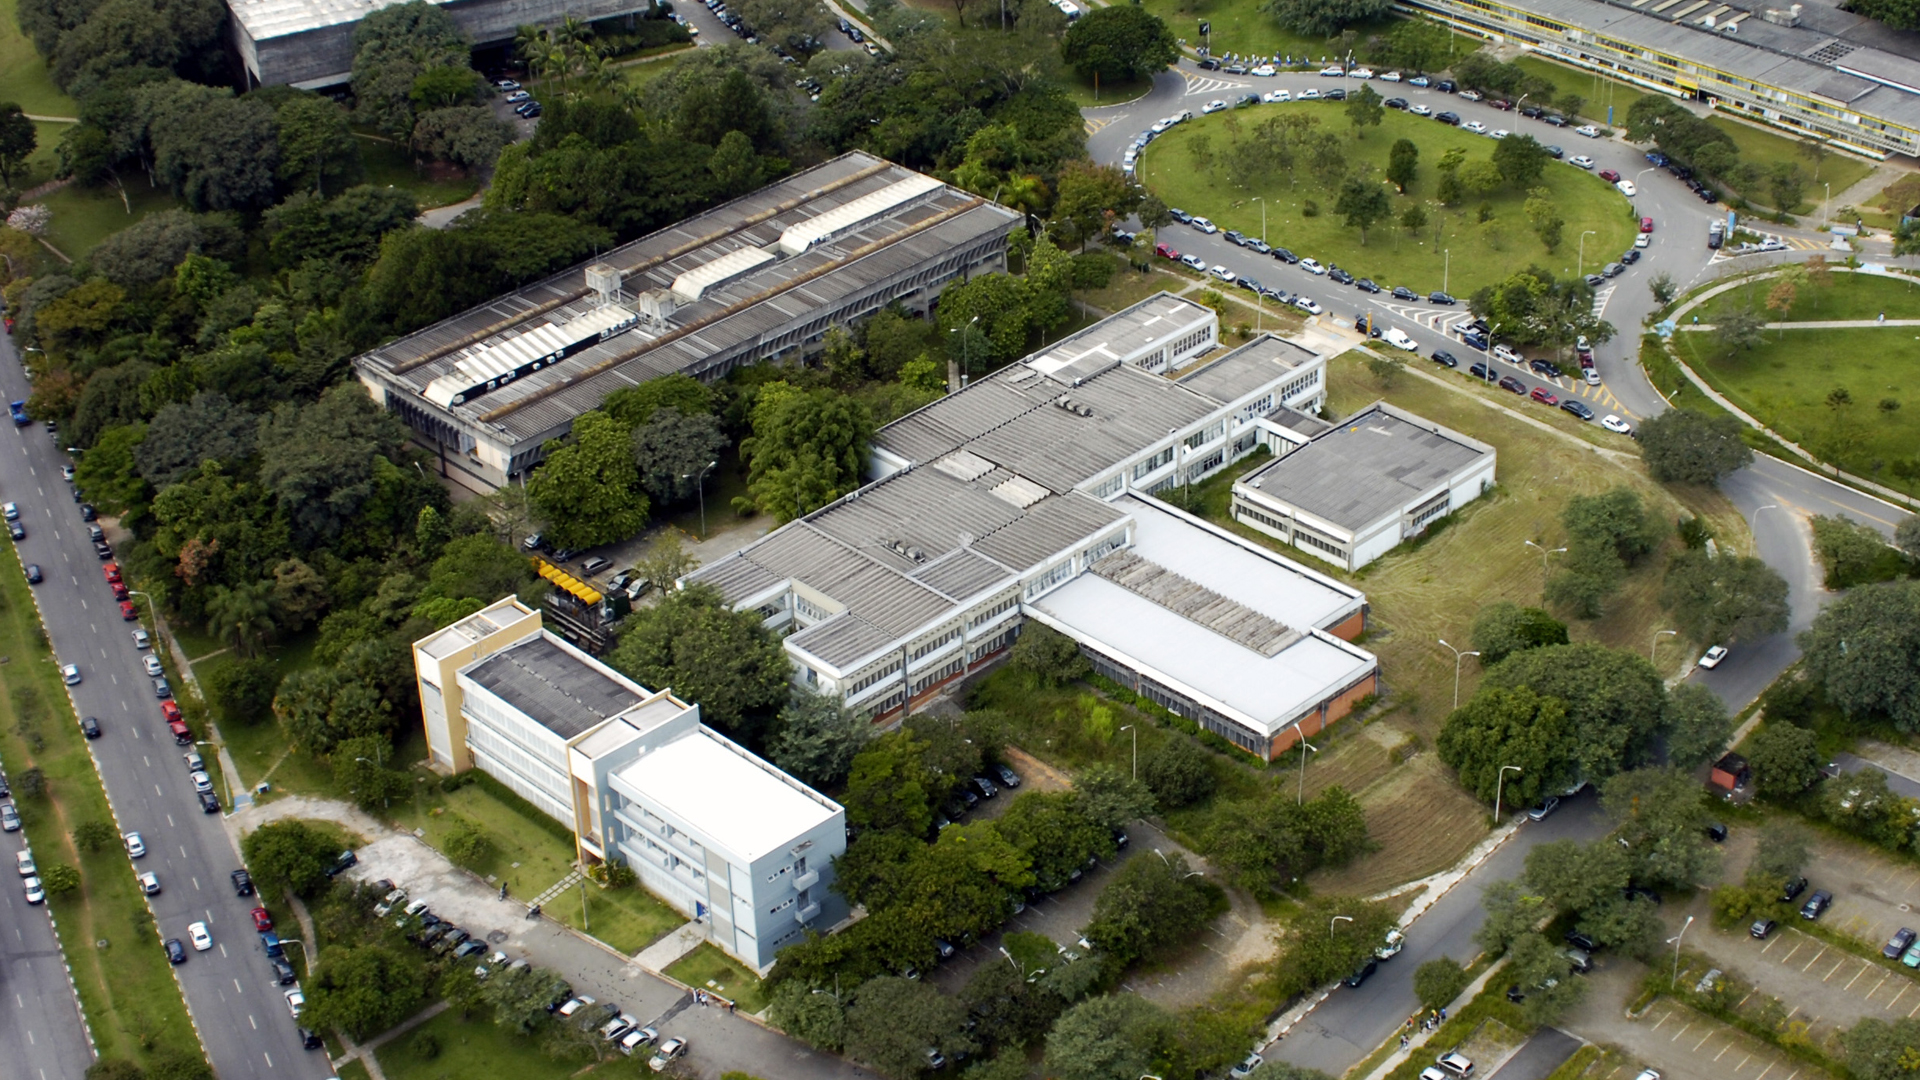
\includegraphics[width=0.95\linewidth]{ime-aerea.jpg}
\\ Institute of Mathematics and Statistics (IME)
\end{figure}
\end{frame}
%------------------------------------------------
\begin{frame}
\frametitle{University of S�o Paulo}
\begin{figure} %POLI%
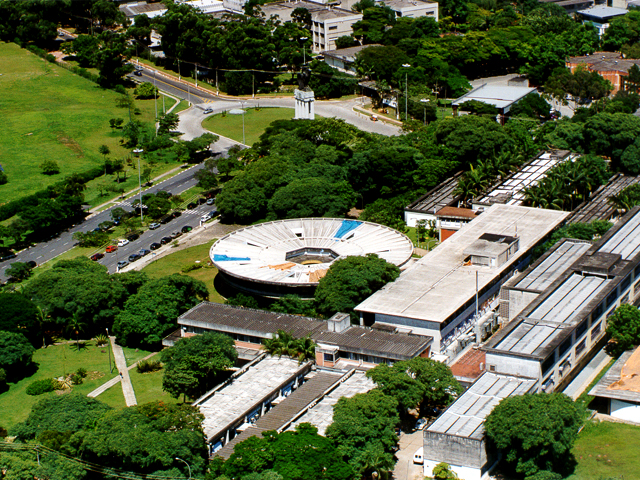
\includegraphics[width=0.75\linewidth]{poli-aerea.jpg}
\\Polytechnic School (POLI)
\end{figure}
\end{frame}
%------------------------------------------------
\begin{frame}
\frametitle{University of S�o Paulo}
\begin{figure} %EACH%
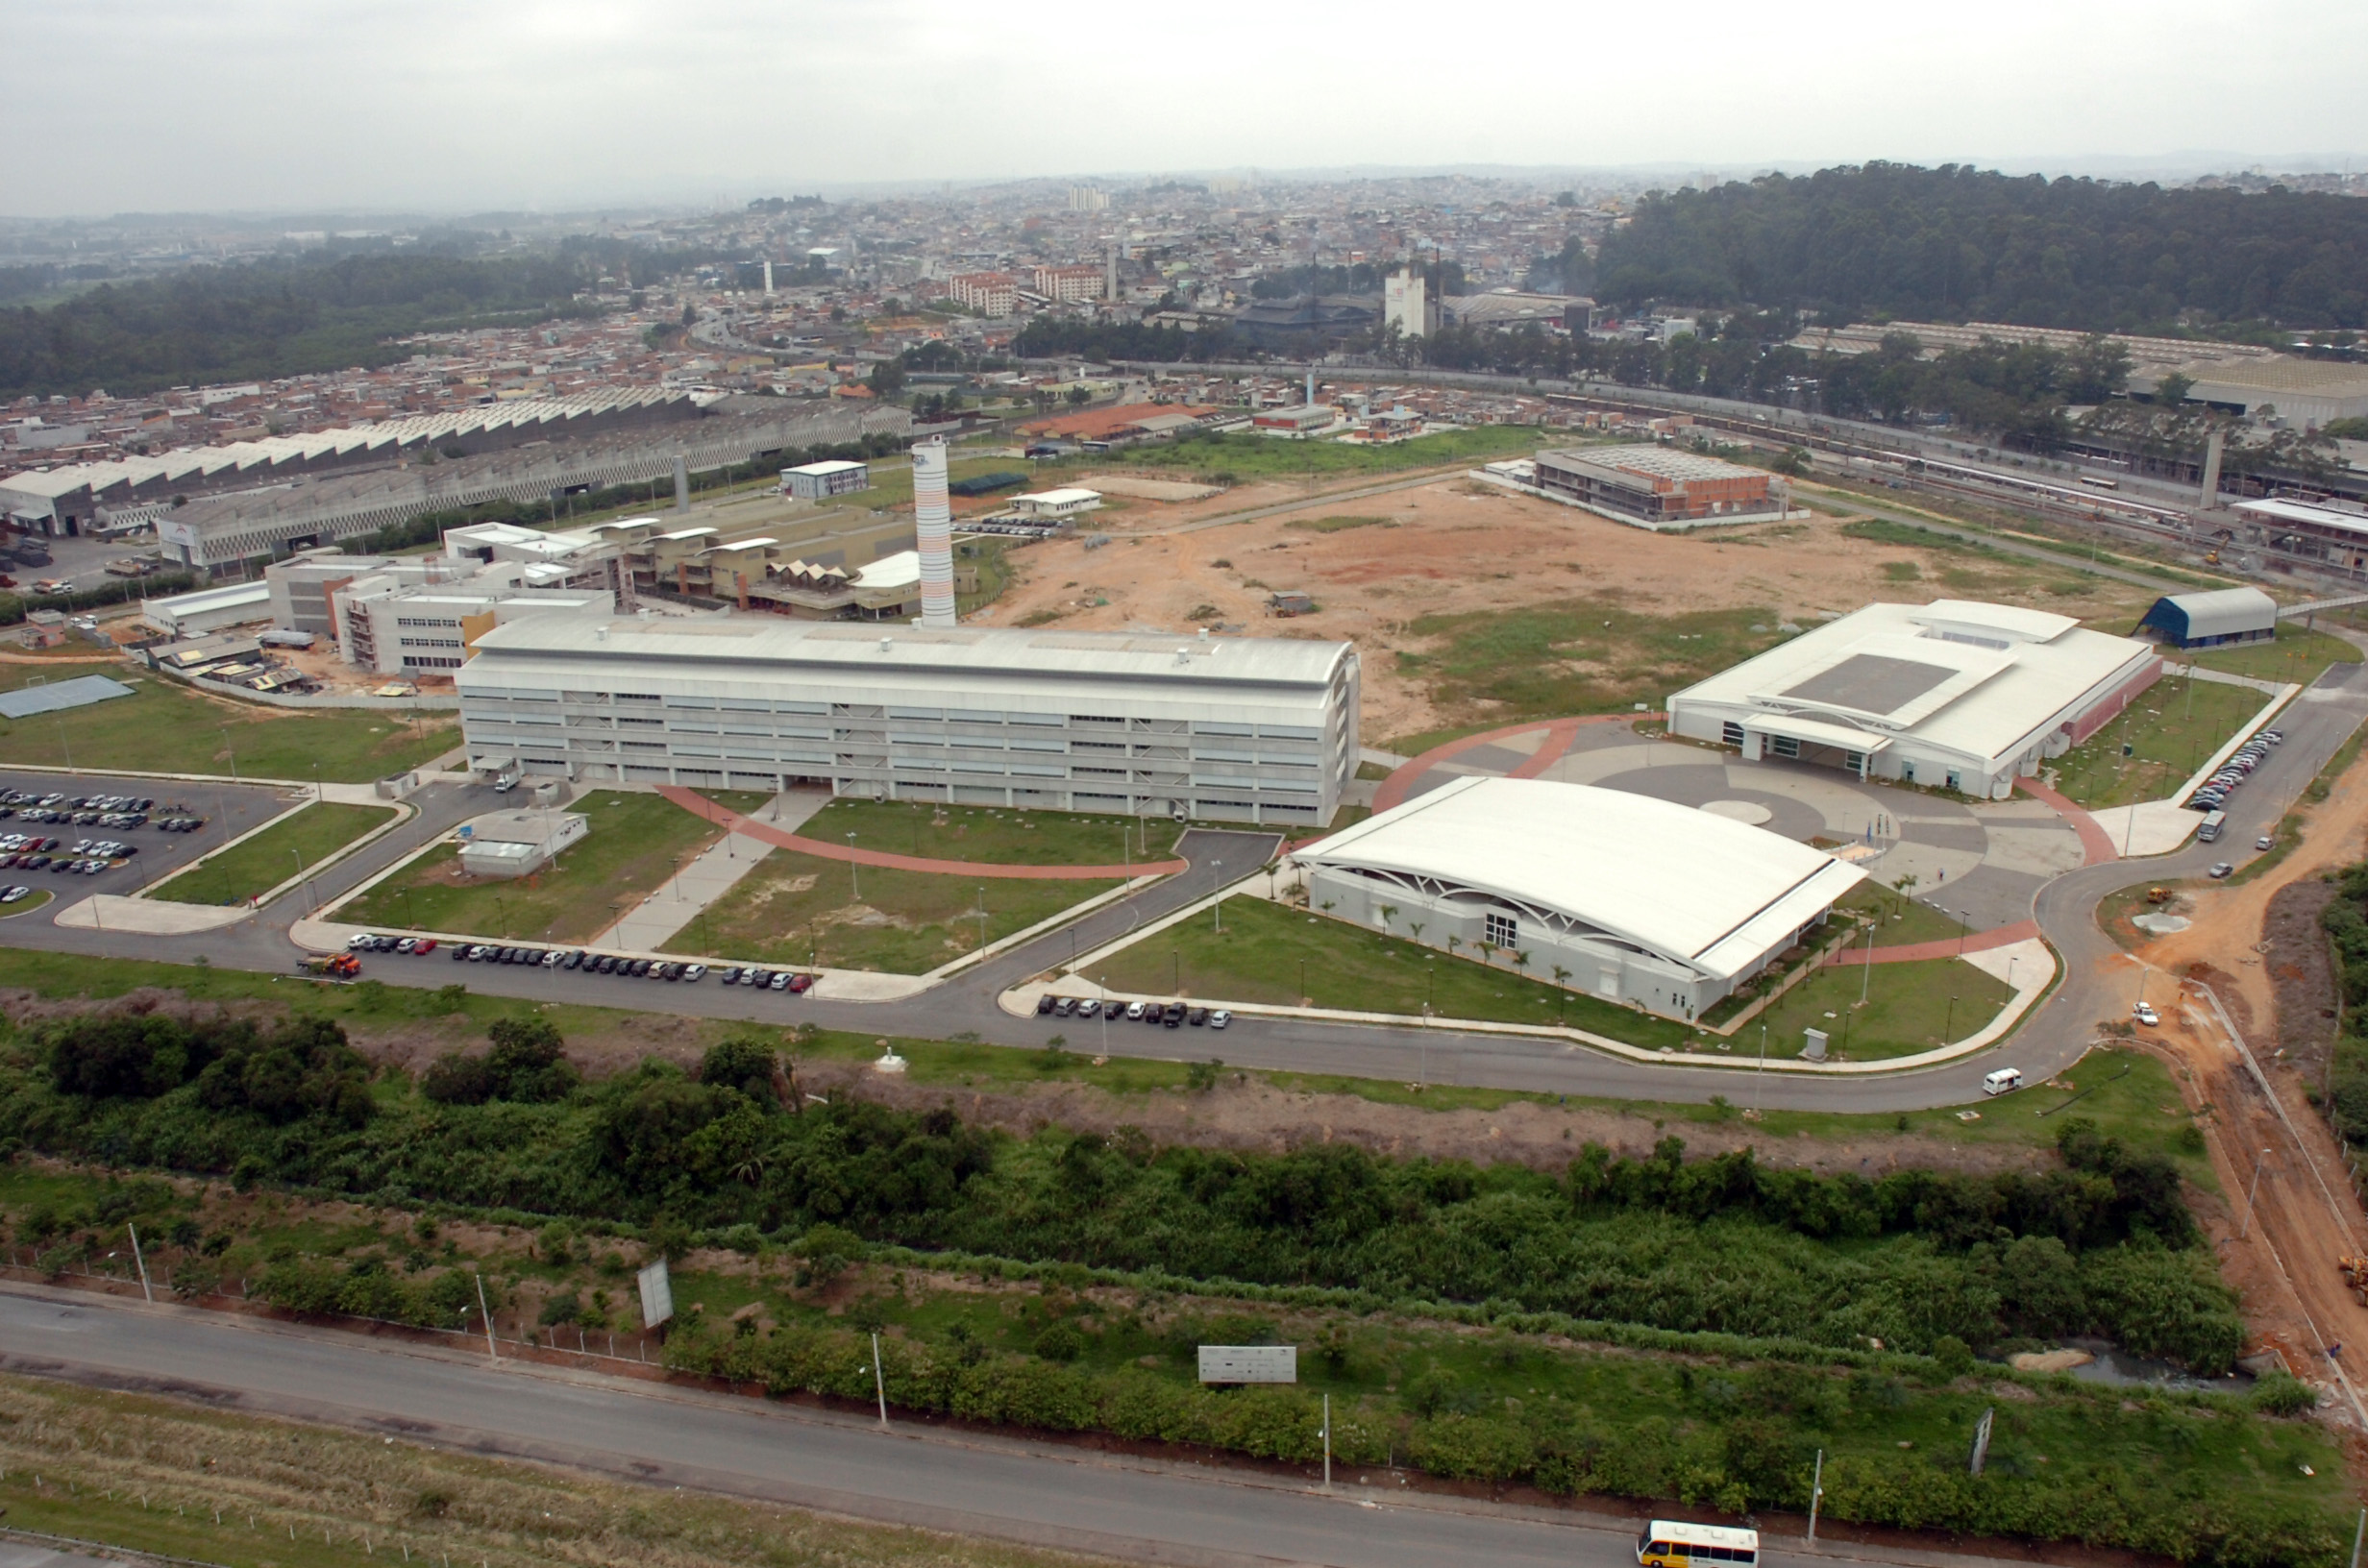
\includegraphics[width=0.85\linewidth]{each-aerea.jpeg}
\\ School of Arts, Sciences and Humanities (EACH)
\end{figure}
\end{frame}
%------------------------------------------------
\begin{frame}
\frametitle{Overview} 
\tableofcontents 
\end{frame}

%----------------------------------------------------------------------------------------
%	PRESENTATION SLIDES
%----------------------------------------------------------------------------------------

%------------------------------------------------
\section{Introduction} 
%------------------------------------------------
\begin{frame}
\frametitle{Introduction}
\begin{block}{Context: logical reasoning and computer programming}
Proposed as fundamental abilities and their introduction in early stages of education has been adopted in an increasing rate
\end{block}
\begin{block}{Problems: introducing it earlier may adress some challenges}
\begin{itemize}
\item Challenges that are currently faced by teacher and students of STEM courses:
	\begin{itemize}
	\item{new software environment (programming environment)}
	\item{new way of describing a problem and it's solution (programming language)}
	\item{learn to solve problems computationally}
	\end{itemize}
\end{itemize}
\end{block}
\end{frame}
%------------------------------------------------ 
\begin{frame}
\frametitle{Introduction}
\begin{block}{Proposals to overcome some of these problems}
\begin{itemize}
\item There are some proposals of using visual systems to support the learning of introductory programming (e.g. Raptor \cite{p1}, Greenfoot\cite{p2}, Scratch \cite{p3} and Alice \cite{p4})
\item Most of Visual Programming (\textbf{VP}) systems allows students to:
	\begin{itemize}
	\item{compile and execute (or interprete) their algorithm with a single click}
	\item{build programs without ``knowing by heart'' the programming language sintax}
	\item{consequently, they may focus their attention to the problem solution}
	\end{itemize}
\end{itemize}
\end{block}
\end{frame}
%------------------------------------------------
\begin{frame}
\frametitle{Introduction}
\begin{block}{This paper approach}
An experiment to evaluate the mental workload during the learning process (VP versus textual) in a web-course context. 
\\To accomplish the analysis we:
\begin{itemize}
\item created two similar web-courses of Introductory Programming
	\begin{itemize}
	\item students were separated into two groups: G1 (visual programming) and G2 (textual programming language)
	\item delivered through Moodle
	\item was an Opened Online Course, not a MOOC since it had 144 students enrolled
	\item same instructional material with differences only concerning the tools
\end{itemize}
\item created a NASA Task Load Index (NASA-TLX) Moodle module for evaluating mental workload
 \end{itemize}
\end{block}
\end{frame}
%------------------------------------------------
\section{Experiment} 
%------------------------------------------------
\begin{frame}
\frametitle{Background: iVProg, VPL and NASA-TLX}
\begin{block}{iVProg}
Visual Programming System to teach algorithms (procedural~programming):
\begin{itemize}
\item firstly deployed in 2009 (based on Alice, from Carnegie Mellon)
\item the second version of iVProg was developed using a framework for Interactive Learning Modules
\item features: 
\begin{itemize}
\item new lines of code with context menu
\item drag-and-drop combined with pointing-and-click to order lines of code
\item edit-in-place for variable names and values
\item automatic evaluation
\item interpret students algorithm with a single click
\end{itemize}
\item iVProg is a Free Software
\begin{itemize}
\item https://github.com/LInE-IME-USP/ivp2java
\end{itemize}
\end{itemize}
\end{block}
\end{frame}
%------------------------------------------------
\begin{frame}
\frametitle{Background: iVProg, VPL and NASA-TLX}
\begin{block}{iVProg}
\begin{figure} %IVPROG%
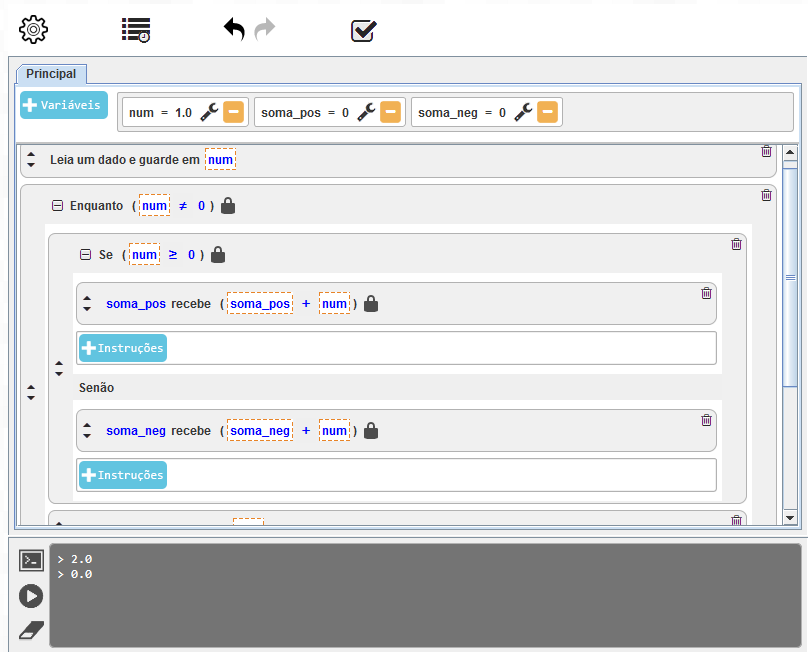
\includegraphics[width=0.70\linewidth]{ivprog.png}
\end{figure}
\end{block}
\end{frame}
%------------------------------------------------
\begin{frame}
\frametitle{Background: iVProg, VPL and NASA-TLX}
\begin{block}{Virtual Programming Lab - VPL}
The VPL system is a Moodle module developed at Universidad de las Palmas Gran Canaria, Spain.
\begin{itemize}
\item is a Free Software for Moodle
\item supports many languages (we used C programming language)
\item automatic evaluation
\item interpret students algorithm with a single click
\item http://vpl.dis.ulpgc.es/index.php/en/
\end{itemize}
\end{block}
\end{frame}
%------------------------------------------------
\begin{frame}
\frametitle{Background: iVProg, VPL and NASA-TLX}
\begin{block}{Virtual Programming Lab - VPL}
\begin{figure} %VPL%
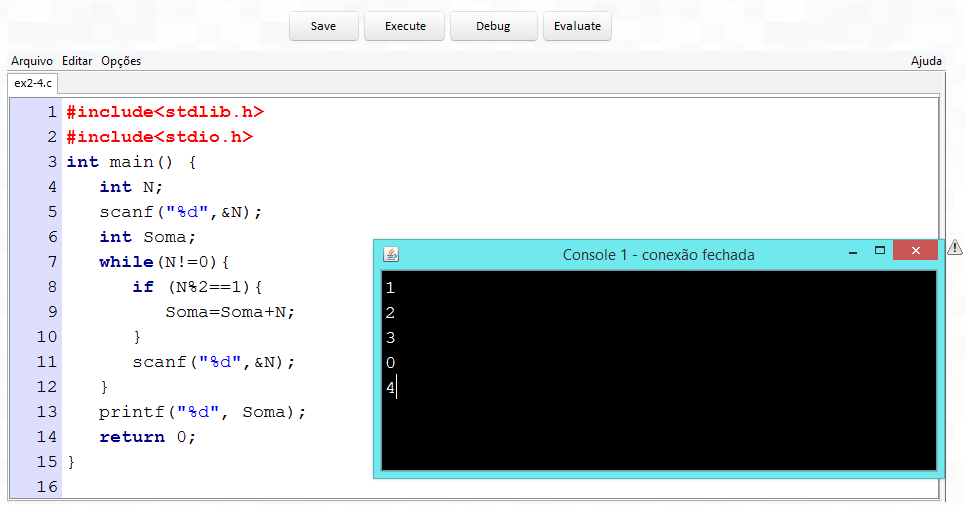
\includegraphics[width=0.90\linewidth]{vpl.png}
\end{figure}
\end{block}
\end{frame}
%------------------------------------------------
\begin{frame}
\frametitle{Background: iVProg, VPL and NASA-TLX}
\begin{block}{NASA-TLX Protocol}
\begin{itemize}
\item Objective: measure workload during the execution of an activity
\item Workload: defined by Hart and Staveland (1988) as a hypothetical construct that represents the cost of someone finishing a task and reaching a certain level of performance.
\item How: by filling up a questionaire with six scales, giving them values and then conducting a pairwise choice between the scales, giving them weights
\item Scales:
\begin{itemize}
\item Mental Demand (MD)
\item Physical Demand (PD)
\item Teporal Demand (TD)
\item Own performance (OP)
\item Effort (EF)
\item Frustration (FR)
\end{itemize}
\end{itemize}
\end{block}
\end{frame}
%------------------------------------------------
\begin{frame}
\frametitle{Background: iVProg, VPL and NASA-TLX}
\begin{block}{NASA-TLX Protocol}
\begin{figure} %NASA TLX%
\includegraphics[width=0.80\linewidth]{nasa-parte1.png}
\\ NASA-TLX $1^{st}$ step: evaluating the demands for each scale after completing one task
\end{figure}
\end{block}
\end{frame}
%------------------------------------------------
\begin{frame}
\frametitle{Background: iVProg, VPL and NASA-TLX}
\begin{block}{NASA-TLX Protocol}
\begin{figure} %NASA TLX%
\includegraphics[width=0.80\linewidth]{nasa-parte2.png}
\\ NASA-TLX $2^{nd}$ step: pairwise choice, giving each scale a weight that represents the importance of each scale while accomplishing a task
\end{figure}
\end{block}
\end{frame}
%------------------------------------------------
\begin{frame}
\frametitle{Experiment setup}
\begin{block}{The course}
\begin{itemize}
\item The course had last for 4 weeks and was delivered fully online
\item Since the environments were Java dependents, students had instruction on how to install Java by video tutorials for Windows and Linux, with Chrome and Firefox examples
\item A small video (our production) with the history of computers were presented
\item The course was organized in 4 blocks
\item Every theoretical content for each block was delivered as hypertext with the very same textual content, but with different images concerning the environment (iVProg and VPL)
\end{itemize}
\end{block}
\end{frame}
%------------------------------------------------
\begin{frame}
\frametitle{Experiment setup}
\begin{block}{Curriculum}
Theoretical and practical content were distributed into the blocks as follows:
\begin{itemize}
\item \textbf{Block 1}: "Algorithms" - definition of algorithms and basic concepts of programming (variables and their types, data input and output etc.)
\item \textbf{Block 2}: "Selection" and it is composed of comments about the previous module, definition of selection with examples.
\item \textbf{Block 3}: "Looping Constructs" and it is composed of comments about the previous module, definition of the looping constructs while, for and repeat
\item \textbf{Block 4}: "Closing" and it is composed of complex activities involving the content of the previous modules and discursive activities related to the course as a whole and a final NASA-TLX activity
\end{itemize}

\end{block}
\end{frame}
%------------------------------------------------
\begin{frame}
\frametitle{Experiment setup}
\begin{block}{Enrollment}
Volunteers registered through web. The propaganda was performed for a short period of time (4 weeks), and mainly restricted to the University of S�o Paulo (USP).
\begin{table}[h]
\begin{tabular}{|l|l|l|l|l|}
\hline
\textbf{Group} & \textbf{System} & \textbf{With experience} & \textbf{Without experience} & \textbf{Total} \\ \hline
\textbf{G1} & iVProg & 31 & 41 & 72 \\ \hline
\textbf{G2} & VPL & 31 & 41 & 72 \\ \hline
\multicolumn{2}{|l|}{\textbf{Total}} & 62 & 82 & 144 \\ \hline
\end{tabular}
\end{table}
\end{block}
\end{frame}
%------------------------------------------------
\begin{frame}
\frametitle{Experiment setup}
\begin{block}{Enrollment: no show}
The number of students that never accessed the system
\begin{table}[h]
\begin{tabular}{|l|l|l|l|l|}
\hline
\textbf{Group} & \textbf{System} & \textbf{With experience} & \textbf{Without experience} & \textbf{Total} \\ \hline
\textbf{G1} & iVProg & 9 & 16 & 25 \\ \hline
\textbf{G2} & VPL & 7 & 14 & 21 \\ \hline
\multicolumn{2}{|l|}{\textbf{Total}} & 16 & 30 & 46 \\ \hline
\end{tabular}
\end{table}
\end{block}
\end{frame}
%------------------------------------------------
\begin{frame}
\frametitle{Experiment setup}
\begin{block}{Enrollment: last week of the course}
A really small number os students had concluded the course and made the activities
\begin{table}[h]
\begin{tabular}{|l|l|l|l|l|}
\hline
\textbf{Group} & \textbf{System} & \textbf{With experience} & \textbf{Without experience} & \textbf{Total} \\ \hline
\textbf{G1} & iVProg & 3 & 3 & 6 \\ \hline
\textbf{G2} & VPL & 2 & 8 & 10 \\ \hline
\multicolumn{2}{|l|}{\textbf{Total}} & 5 & 11 & 16 \\ \hline
\end{tabular}
\end{table}
\end{block}
\end{frame}
%------------------------------------------------
\begin{frame}
\frametitle{Methodology}
\begin{block}{Data analysis}
\begin{itemize}
\item NASA-TLX: Wilcoxon-Mann-Whitney (WMW) test and comparisons with medians
\begin{itemize}
\item reason: low number of respondents, besides the apparent nonsymmetrical distribution of data
\item brief: WMW test consists of defining ranks based on the samples values.~The higher the sample ranks, the higher is the values in the distribution
\item hypothesis:
\begin{itemize}
\item  $H_0: distribution_{G1} = distribution_{G2}$
\item  $H_1: distribution_{G1} < distribution_{G2}$
\item exception: scale \emph{Own Performance} (OP), where $H_1: distribution_{G1} > distribution_{G2}$
\end{itemize}
\end{itemize}
\item Activities: quantitative analysis describing the number of attempts
\end{itemize}
\end{block}
\end{frame}
%------------------------------------------------
\begin{frame}
\frametitle{Results}
\begin{block}{NASA-TLX Block 1}
\begin{figure} %NASA TLX%
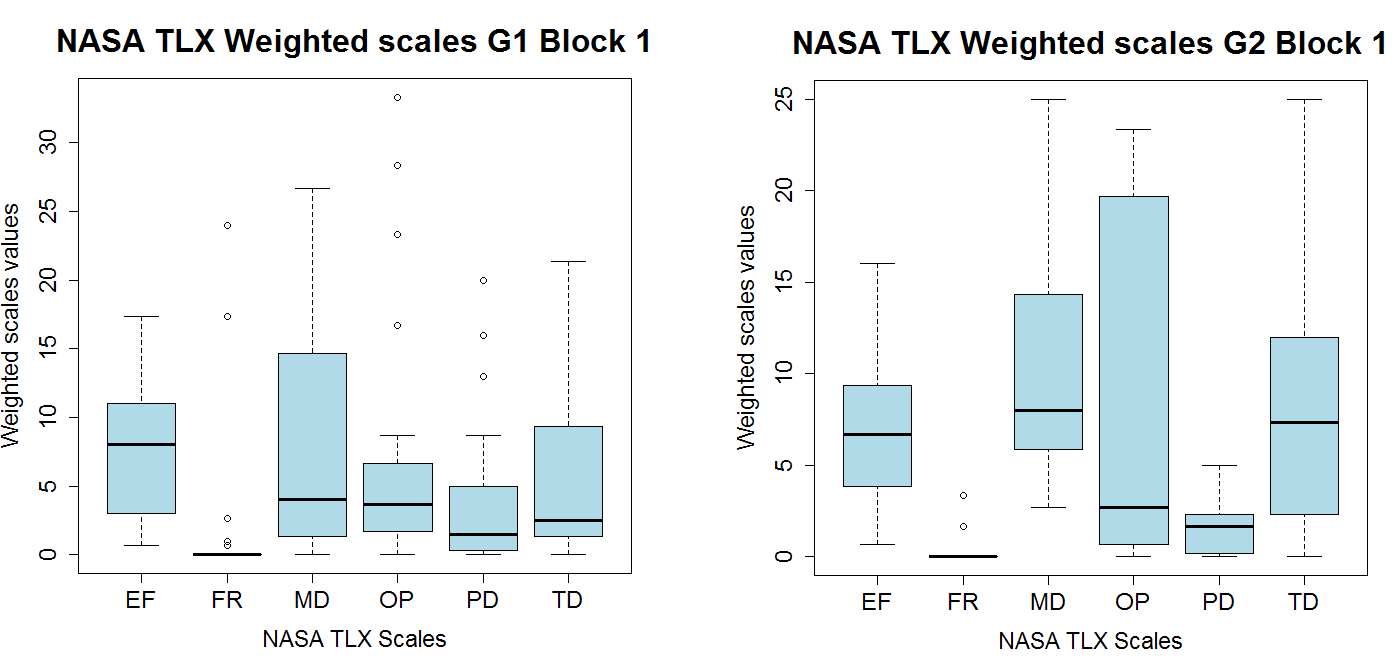
\includegraphics[width=0.9\linewidth]{block1.png}
\begin{table}[h]
\begin{tabular}{|l|l|l|l|l|l|l|}

\hline
 & \textbf{EF} & \textbf{FR} & \textbf{MD} & \textbf{OP} & \textbf{PD} & \textbf{TD} \\ \hline
\emph{p}-value & 0.6409 & 0.6676 & 0.1167 & 0.3002 & 0.8272 & 0.1132 \\ \hline
\end{tabular}
\end{table}
\end{figure}
\end{block}
\end{frame}
%------------------------------------------------
\begin{frame}
\frametitle{Results}
\begin{block}{Attempts Block 1}
\begin{itemize}
\item G2 group: (C+VPL, textual programming), the maximum number of attempts were 15 times and it was not uncommon to find a number greater than five attempts
\item G1 group: (iVProg) used 4 attempts at most (only 1 student), more than that, the most common situation was the student submit the correct answer in first trial
\end{itemize}
\end{block}
\end{frame}
%------------------------------------------------
\begin{frame}
\frametitle{Results}
\begin{block}{NASA-TLX Block 2}
\begin{figure} %NASA TLX%
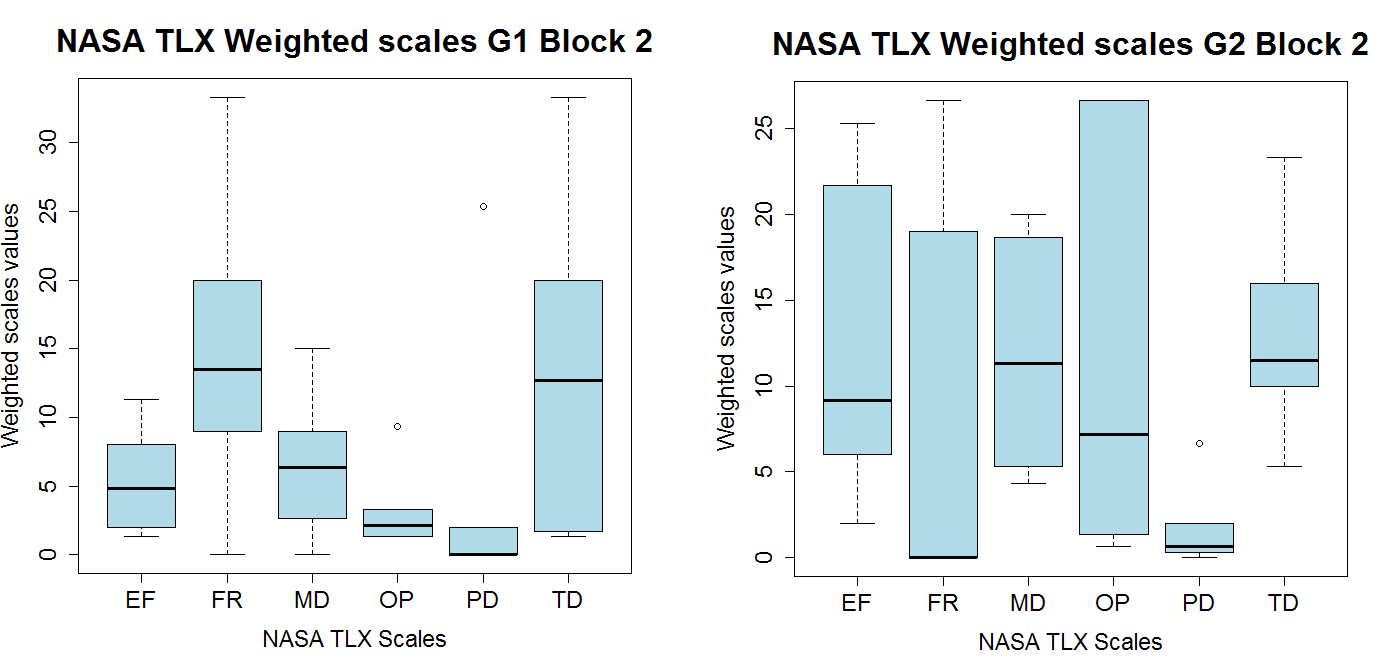
\includegraphics[width=0.9\linewidth]{block2.png}
\begin{table}[h]
\begin{tabular}{|l|l|l|l|l|l|l|}
\hline
 & \textbf{EF} & \textbf{FR} & \textbf{MD} & \textbf{OP} & \textbf{PD} & \textbf{TD} \\ \hline
\emph{p}-value & 0.07441 & 0.8935 & 0.1473 & 0.2071 & 0.2023 & 0.532 \\ \hline
\end{tabular}
\end{table}
\end{figure}
\end{block}
\end{frame}
%------------------------------------------------
\begin{frame}
\frametitle{Results}
\begin{block}{Attempts Block 2}
\begin{itemize}
\item G2 group: the maximum number of attempts to solve a problem was 12 and the most common situation is the use of 5 attempts
\item G1 group:maximum number of attempts was 4 and the most common situation was students sending the correct answer in their first trial \end{itemize}
\end{block}
\end{frame}
%------------------------------------------------
\begin{frame}
\frametitle{Results}
\begin{block}{NASA-TLX Block 3}
\begin{figure} %NASA TLX%
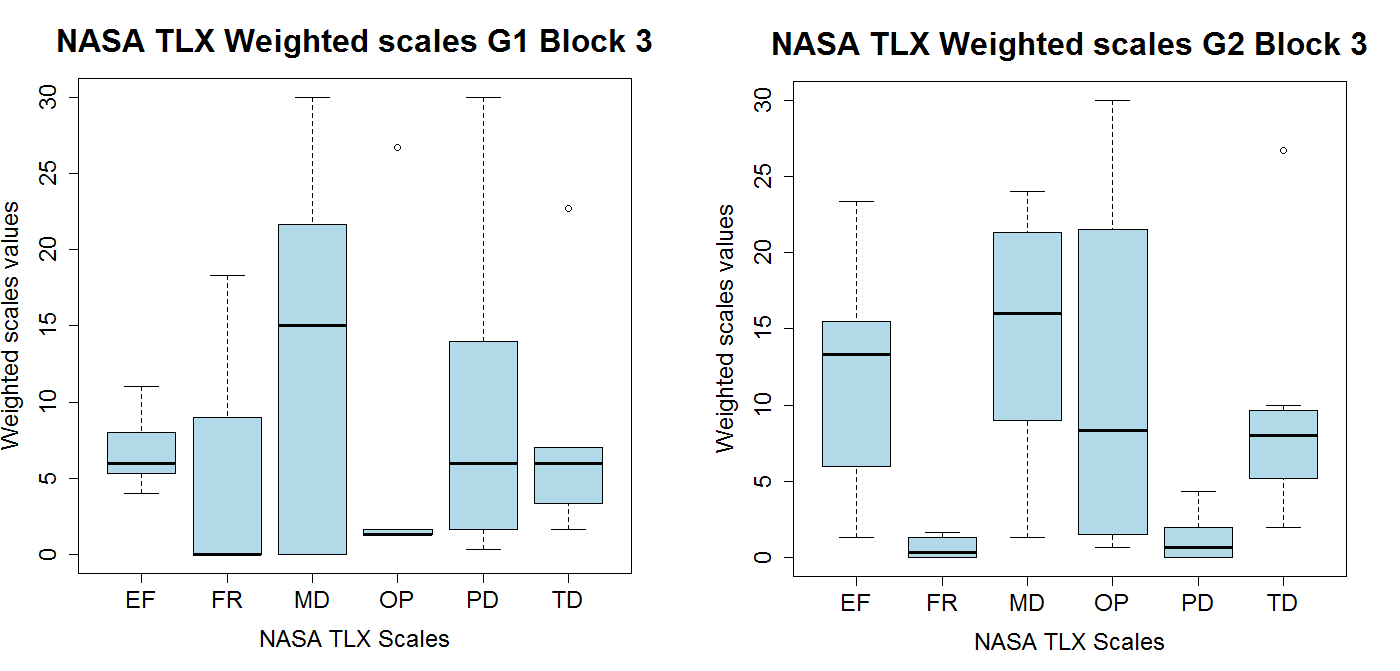
\includegraphics[width=0.9\linewidth]{block3.png}
\begin{table}[h]
\begin{tabular}{|l|l|l|l|l|l|l|}
\hline
 & \textbf{EF} & \textbf{FR} & \textbf{MD} & \textbf{OP} & \textbf{PD} & \textbf{TD} \\ \hline
\emph{p}-value & 0.1452 & 0.6028 & 0.4353 & 0.7435 & 0.9642 & 0.6028 \\ \hline
\end{tabular}
\end{table}
\end{figure}
\end{block}
\end{frame}
%------------------------------------------------
\begin{frame}
\frametitle{Results}
\begin{block}{Attempts Block 3}
\begin{itemize}
\item G2 group: the number of submissions was slightly higher than in G1 (6 students), however, the number of attempts reached the maximum of 17
\item G1 group: regarding the number of submissions for G1 few students (5) did the activities, however, their submission was correct on only 1 attempt for all the students
\end{itemize}
\end{block}
\end{frame}
%------------------------------------------------
\section{Discussion, conslusions and future work}
%------------------------------------------------

\begin{frame}
\frametitle{Discussion, conclusions and future work}
\begin{block}{Discussion: NASA-TLX}
The NASA TLX also showed that, in some cases, users have shown a little bit frustrated during the execution of the proposed tasks.
In order to understand this phenomenon and, moreover, to collect qualitative data about the web-course we designed a simple online survey
\begin{itemize}
\item (unfortunately) the number of NASA TLX submissions for the forth block were not sufficient to make any comparison 
\item NASA TLX also showed that, in some cases, users have shown a little bit frustrated during the execution of the proposed tasks
\end{itemize}
To understand this phenomenon and, moreover, to collect qualitative data about the web-course we designed a simple online survey
\end{block}
\end{frame}

%------------------------------------------------
\begin{frame}
\frametitle{Discussion, conclusions and future work}
\begin{block}{Discussion: online survey}
\begin{enumerate}
\item If you have not accessed the course system or did not accomplished the module I could share the reason with us? If yes, fill out the form below telling us why.
\item If you did the activities and read the instructional material, do you have any suggetion of improvement to the environment or to the material?
\item What is your opinion about the tool used to create algorithms?
\end{enumerate}
\end{block}

\begin{block}{Discussion: answers}
The survey questionnaire was answered by 26 students (23 accessed the course and 3 did not). The main reason to frustrations were problems with the Java applet technology and the difficulties with its configuration.
\end{block}
\end{frame}
%------------------------------------------------
\begin{frame}
\frametitle{Discussion, conclusions and future work}
\begin{block}{Discussion: perceptions and considerations}
Considering all collected data, from NASA TLX, activities log, and the survey, we can observe that visual programming is a good model to teach algorithms and programming. However the low number of respondents do not allow stronger assertions.
\end{block}
\end{frame}

\begin{frame}
\frametitle{Discussion, conclusions and future work}
\begin{block}{Future work}
\begin{itemize}
\item Since the reduced number of enrolled students prevented us of any statistical conclusions, we intend to perform a new course edition, this time as MOOC
\item Analyse if a new version of iVProg, now implemented using HTML5 technology can reduce the students frustrations with Java security issues
\item Besides, this first course edition comparing visual with textual programming arose several questions that must be investigated in future.
	\begin{itemize}
	\item One of them is how to compare the effective learning. Is it possible to compare both models?
	\end{itemize}
\end{itemize}

\end{block}
\end{frame}
%------------------------------------------------

\begin{frame}
\frametitle{Discussion, conclusions and future work}
Questions?
\begin{block}{Presenter}
Le�nidas de Oliveira Brand�o\\
leo@ime.usp.br\\
DCC - IME - USP\\
Room 212 - Block C - 55 11 3091 9691\\
Rua do Mat�o, 1010 - Cidade Universit�ria - S�o Paulo - SP\\

\end{block}

\end{frame}
%------------------------------------------------

\begin{frame}
\frametitle{References}
\footnotesize{
\begin{thebibliography}{99} % Beamer does not support BibTeX so references must be inserted manually as below
\bibitem[Carlisle]{p1} [1] Carlisle, M. C. (2009)
\newblock Raptor: a visual programming environment for teaching object-oriented programming
\newblock \emph{Journal of Computing Sciences in Colleges}, Vol. 24, issue 4, April 2009, pp. 275-281.

\bibitem[K�lling]{p2}[2] K�lling, M. (2010)
\newblock The Greenfoot Programming Environment
\newblock \emph{Transactions on Computing Education (TOCE)}, Vol. 10, issue 4, November 2010.

\bibitem[Maloney et al.]{p3}[3] Maloney, J., Resnick, M., Rusk, N., Silverman, B., Eastmond, E. (2010)
\newblock The Scratch programming language and environment
\newblock \emph{Transactions on Computing Education (TOCE)}, Vol. 10, issue 4, November 2010.

\bibitem[Cooper et al.]{p4}[4] Cooper, S., Dann, W., Pausch, R. (2000)
\newblock Alice: a 3-D tool for introductory programming concepts
\newblock \emph{Journal of Computing Sciences in Colleges}, Vol. 15, issue 5, May 2000, pp.107-116.
\end{thebibliography}
}
\end{frame}
%------------------------------------------------
\begin{frame}
\frametitle{References}
\footnotesize{
\begin{thebibliography}{99} % Beamer does not support BibTeX so references must be inserted manually as below
\bibitem[Hart and Staveland]{p5}[5] Hart, S. G., Staveland, L. E.  (1988)
\newblock Development of NASA-TLX (Task Load Index): Results of Empirical and Theoretical Research
\newblock \emph{P. A. Hancock and N. Meshkati (Eds.) Human Mental Workload.} Amsterdam: North Holland Press.
\end{thebibliography}
}
\end{frame}
%----------------------------------------------------------------------------------------

\end{document} 